
Ideally one would measure a two-dimensional luminosity density,
$L(x,y)$, for each cluster, as in Equation~(\ref{eq:ratedenom}).
However, the large background makes this difficult. For our purpose
(which is to account for variations in control time with radius), it
is sufficient to assume the clusters have a circularly symmetric
luminosity distribution, $L(r)$. For each cluster, we sum the total
luminosity in annuli of width 0.1~Mpc. For nearly all clusters there
is a clear overdensity relative to the background out to $r \sim
0.3$~Mpc (Fig.~\ref{fig:allprofiles_all}). Beyond $0.3$~Mpc, the
luminosity measurement is dominated by background noise for most
clusters. This might appear to be a problem; we wish to characterize
the cluster luminosities out to $r \gtrsim 0.7$~Mpc, the area over
which we searched for SNe. In fact, it is only necessary to accurately
measure the \emph{average} luminosity profile over the full area (the
denominator of Eq.~\ref{eq:rate} is the sum of the cluster
luminosities, weighted by control time). Averaging all 25 clusters,
there is a significant measurement of the luminosity profile out to
$>0.5$~Mpc (Fig.~\ref{fig:avgprofile_mult}, left panels), and the
average cluster luminosity within $r<0.6$~Mpc has an error of $12\%$
(statistical only) and $\sim 20\%$ (statistical $+$ cosmic variance),
below the Poisson error in the number of SNe detected.

%%%%%%%%%%%%%%%%%%%%%%%%%%%%%%%%%%%%%%%%%%%%%%%%%%%%%%%%%%%%%%%%%%%%
% FIGURES: LUMINOSITY PROFILES -- ALL CLUSTERS                     %
%%%%%%%%%%%%%%%%%%%%%%%%%%%%%%%%%%%%%%%%%%%%%%%%%%%%%%%%%%%%%%%%%%%%
\begin{figure}[tp]
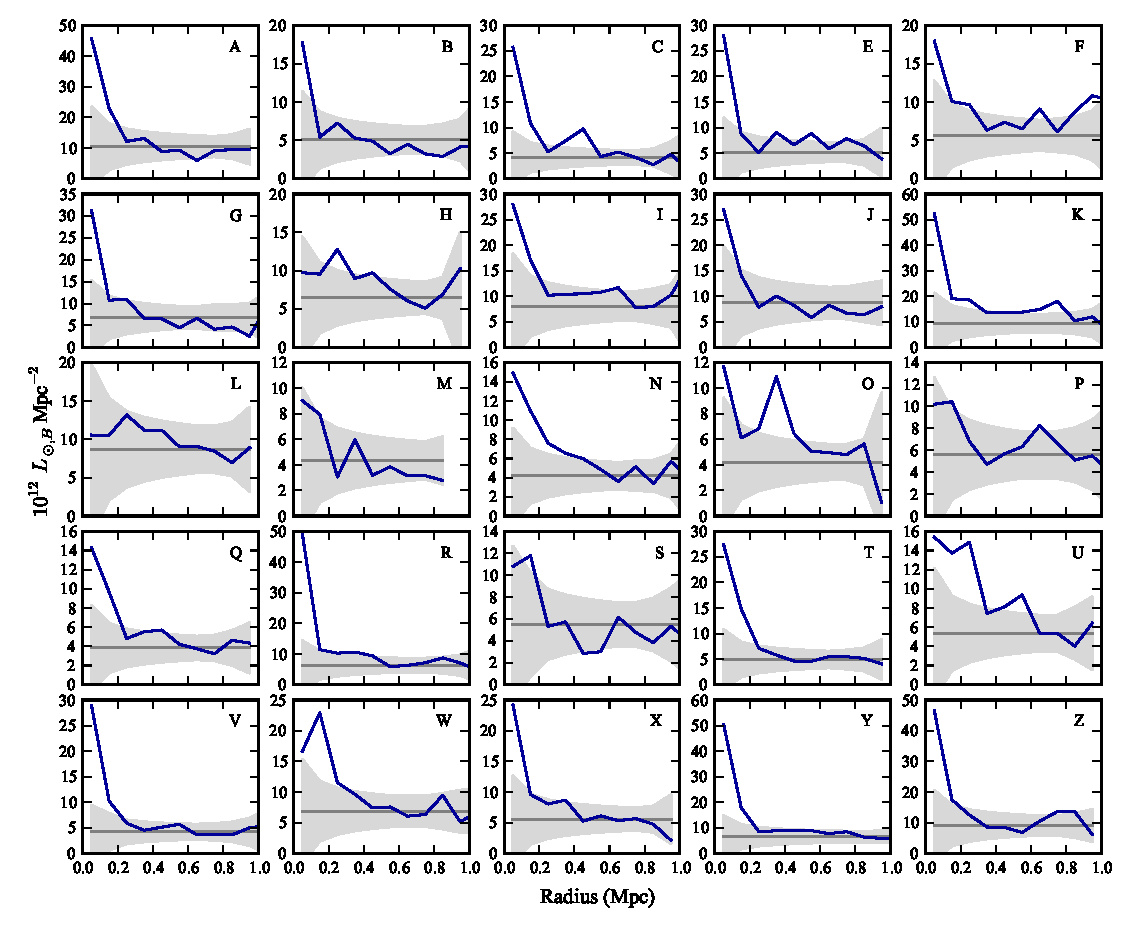
\includegraphics[angle=270]{figures/clrate/allprofiles_all.eps}
\caption[Luminosity profiles of 25 clusters]{Luminosity profiles
of all 25 clusters. The grey line and shaded region represents the
estimated background luminosity density and uncertainty on the
background at each radius. The background uncertainty decreases
with radius because larger annuli sample more area. At large radii,
the uncertainty increases again because only some parts of the outer
annuli (on the deepest part of the image) are used in computing the
luminosity. \label{fig:allprofiles_all}}
\end{figure}

\begin{figure}[tp]
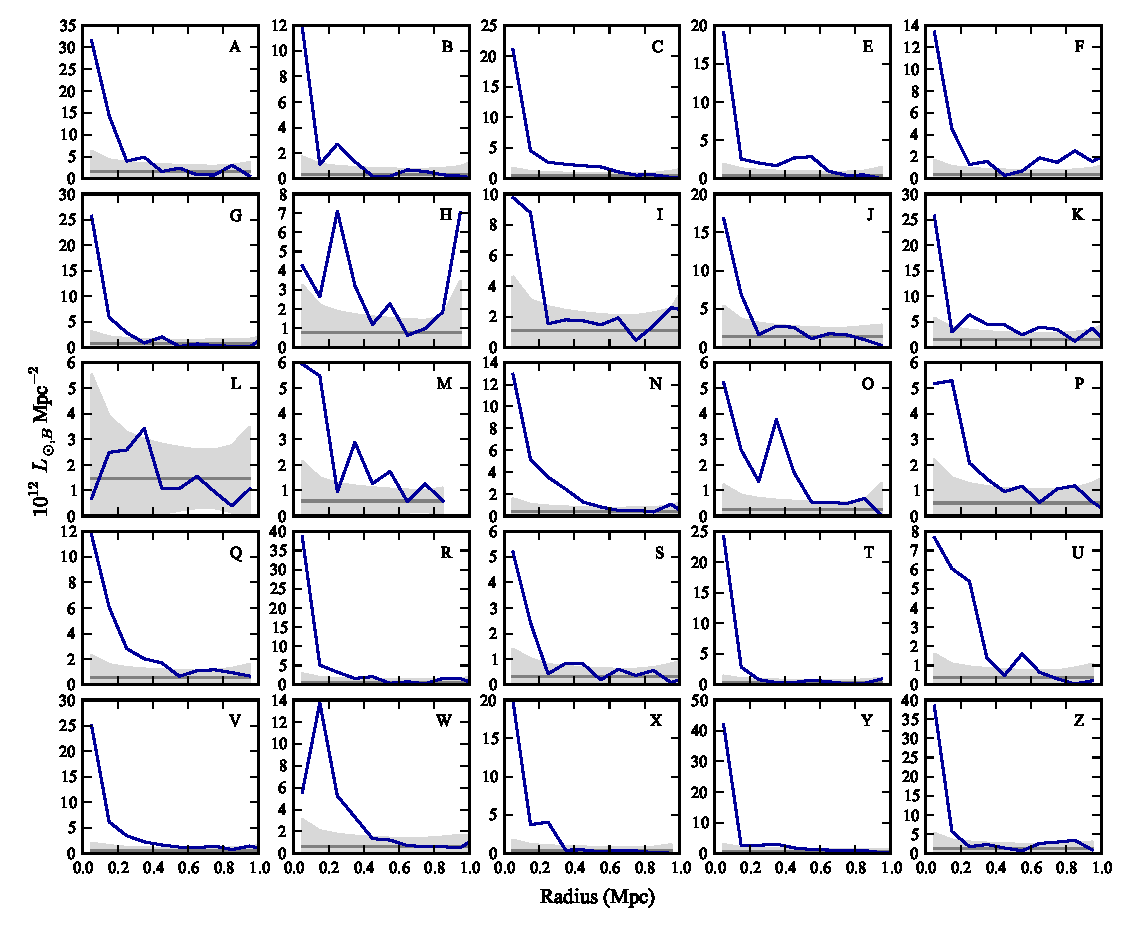
\includegraphics[angle=270]{figures/clrate/allprofiles_rs.eps}
\caption[Luminosity profiles of 25 clusters -- red-sequence galaxies]
{Same as Figure~\ref{fig:allprofiles_all}, but for galaxies on the red
sequence only. \label{fig:allprofiles_rs}}
\end{figure}

\begin{figure}[tp]
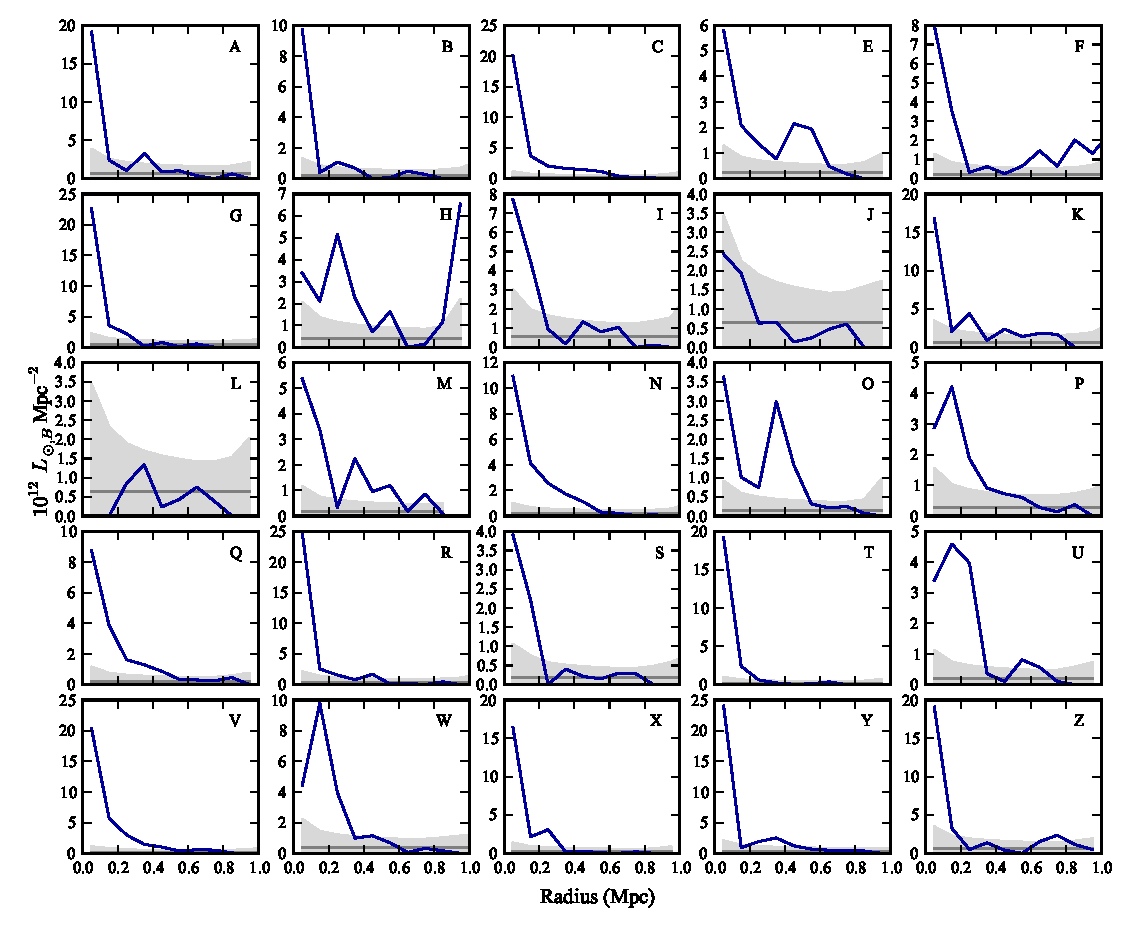
\includegraphics[angle=270]{figures/clrate/allprofiles_rse.eps}
\caption[Luminosity profiles of 25 clusters -- red-sequence elliptical
  galaxies] {Same as Figure~\ref{fig:allprofiles_all}, but for {\it
    elliptical} galaxies on the red sequence
  only. \label{fig:allprofiles_rse}}
\end{figure}

%%%%%%%%%%%%%%%%%%%%%%%%%%%%%%%%%%%%%%%%%%%%%%%
% FIGURE: AVERAGE CLUSTER LUMINOSITY PROFILES %
%%%%%%%%%%%%%%%%%%%%%%%%%%%%%%%%%%%%%%%%%%%%%%%

\begin{figure}[tb]
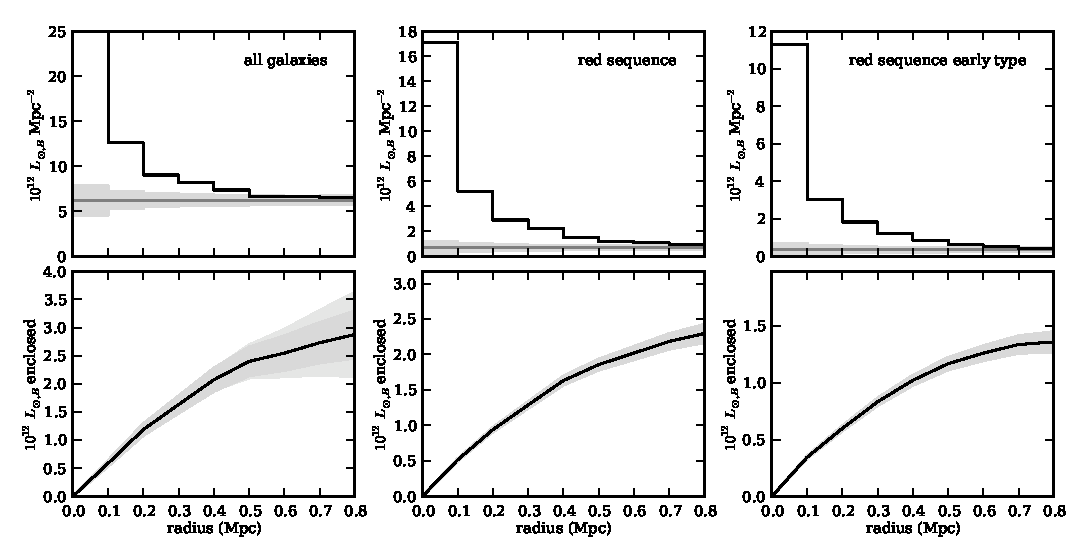
\includegraphics[width=\textwidth]{figures/clrate/avgprofile_mult.eps}
\caption[Average luminosity profile of the 25 clusters.]
{Average luminosity profile of the 25 clusters. {\it Top row:}  
Average luminosity density in the cluster fields in annuli of width
0.1~Mpc extending out from the cluster center. The grey line and
shaded region show the estimated ``background'' luminosity in each
annulus and the error on that background, respectively. The darker
grey region is the statistical-only error, while the light grey is the
statistical $+$ cosmic variance error, added in quadrature. {\it
Bottom row:} The total enclosed luminosity as a function of radius,
derived by subtracting the background from the total luminosity
density in each bin in the top row plot. The \emph{left plots} include
galaxies of all colors and morphologies, while the \emph{center plots}
include only galaxies with $i_{775}-z_{850}$ colors within $\pm
0.2$~mag of the red sequence in their respective clusters. The \emph{right
plots} include only galaxies that satisfy the color requirement and
also have $z_{850} < 24$ and are morphologically early type. By
excluding bluer galaxies (center and right plots) the background (and
error) is reduced dramatically.\label{fig:avgprofile_mult}}
\end{figure}

Beyond $r<0.6$~Mpc, the control time is generally small (that is,
there are few observations covering the outskirts of the clusters) and
the cluster luminosity density is low, meaning that these regions will
not contribute greatly to the rate measurement. Still, we include
these regions in our rate calculation, using the entirely reasonable
prior that the luminosity density is decreasing with radius past
$r<0.6$~Mpc. How rapidly the luminosity density decreases will not
have a significant impact on the result, but as a convenient analytic
description we fit a $\beta$-model of the form
\begin{equation}
L(r) = \frac{\Sigma_0}{(1+(r/r_{\rm core})^2)^\beta}
\end{equation}
over the range $r<0.6$~Mpc and apply this function at $r>0.6$~Mpc. The
data are well-fit by this model, with best-fit parameters $r_{\rm
core} = 0.074$~Mpc and $\beta= 0.91$. Varying this model luminosity by
$\Delta\Sigma_0 = \pm 20\%$ (easily enclosing the allowed range of
$L(r)$) only changes our results by $\pm 4\%$. This and other
systematic uncertainties are summarized in
Table~\ref{tab:clrate_sys}.

%We have chosen to be agnostic with regard to the shape of the luminosity
%profile, using the actual measured luminosities, rather
%than a functional form fit to the data. 


%%%%%%%%%%%%%%%%%%%%%%%%%%%%
% average luminosity table %
%%%%%%%%%%%%%%%%%%%%%%%%%%%%

\begin{table}[tbhp]
\caption{\label{tab:lum_avg} Average cluster luminosities within $r < 0.6$~Mpc}
\begin{center}
\begin{footnotesizetabular}{lccccc}
\hline
\hline
       &     &           & All galaxies          & RS galaxies & 
RSE galaxies \\
Subset & $N$ & $\bar{z}$ & ($10^{12} L_{\odot,B}$) & ($10^{12} L_{\odot,B}$) &
($10^{12} L_{\odot,B}$) \\
\hline
X-ray & 9 & 1.20 & $ 2.86 \pm  0.54 \pm  0.45$ & $ 2.42 \pm  0.16 \pm  0.05$ & $ 1.47 \pm  0.12 \pm  0.02$ \\
IR-Spitzer & 7 & 1.30 & $ 2.85 \pm  0.70 \pm  0.52$ & $ 1.83 \pm  0.24 \pm  0.07$ & $ 0.96 \pm  0.16 \pm  0.03$ \\
Optical & 9 & 1.00 & $ 1.99 \pm  0.37 \pm  0.32$ & $ 1.75 \pm  0.08 \pm  0.03$ & $ 1.29 \pm  0.06 \pm  0.01$ \\[0.1in]
$z<1.2$ & 14 & 1.02 & $ 2.14 \pm  0.31 \pm  0.33$ & $ 1.79 \pm  0.07 \pm  0.03$ & $ 1.28 \pm  0.05 \pm  0.01$ \\
$z>1.2$ & 11 & 1.32 & $ 3.06 \pm  0.58 \pm  0.54$ & $ 2.31 \pm  0.19 \pm  0.07$ & $ 1.23 \pm  0.14 \pm  0.04$ \\[0.1in]
All & 25 & 1.15 & $ 2.54 \pm  0.31 \pm  0.42$ & $ 2.02 \pm  0.09 \pm  0.05$ & $ 1.26 \pm  0.07 \pm  0.02$ \\
\hline
\end{footnotesizetabular}

\end{center}
{\footnotesize
{\bf Note.} --- ``RS'': galaxies within $\pm 0.2$~mag
of the cluster red sequence. ``RSE'': galaxies fulfilling the ``RS''
requirement, and also $z_{850} < 24$, and morphologically
early-type. The first and second confidence intervals are the
statistical error and cosmic variance error, respectively. These
luminosities do not include the faint-galaxy correction $C$.}
\end{table}

